\section{Introduction}

%
% Thanks to Martha Field for discussion on adapting mammalian cells
% to synthetic media.
%
FBA has become extremely popular, in part, due to its simplicity in
calculating reasonably accurate microbial fluxes. For many microbes, a
simple synthetic environment where all chemical species are known
suffices to allow proliferation. Additionally, it has been found that
their biological objectives can be largely expressed as linear
objectives of fluxes.  Neither of these assumptions necessarily hold
for mammalian cells growing \emph{in vitro} or \emph{in vivo}, and in
particular the environment is far more complex for mammalian cell
cultures, which have to undergo gradual metabolic adaptation via
titration to grow on synthetic media. In what follows we first discuss
the MoMA algorithm since it is heavily extended in order to allow us
to use expression data for the estimation of flux data.

\hl{The following subsection on MoMA will probably be moved to the
preceding chapter which also makes use of MoMA.}

\subsection{MoMA: Minimization of Metabolic Adjustment}

The minimization of metabolic adjustment (MoMA) method \cite{Segre2002}, 
which is framed as a least-squares optimization problem, is typically employed
to calculate the flux vector of an \emph{in silico} organism after a
mutation by minimizing the distance between the wild-type flux and the
mutant flux. The biological intuition is that the organism has not had
time to adapt to the restricted metabolic capacity and will maintain a
similar flux to the wild-type (WT) except where the perturbations due
to the mutation dictate necessary alterations in fluxes \hl{(cite ROOM)}.

Suppose $\mathbf{a}$ is the WT flux vector obtained by an optimization procedure, 
such as min-norm FBA (flux balance analysis), empirical measurements, or a
combination of these. Then for an undetermined flux vector $\mathbf{v}$ in a model 
with $N$ reactions the optimization objective can be expressed as
\[ \textnormal{minimize}\ \sum^N_{i=1}(v_i-a_i)^2 \]
subject to the stoichiometric constraints $\mathbf{S v} = \mathbf{0}$
where $\mathbf{v} = (v_1, \ldots, v_N)^T$. This assumes that each $a_i$ is measured,
but it is also possible and sometimes even more useful to employ this objective when only
a subset of the $a_i$ are measured (if $a_i$ is not measured for some $i$, then we omit
$(v_i-a_i)^2$ from the objective). In metabolomics, for instance, it is always the case in experiments with 
labeled isotope tracers that only a relatively small subset of all fluxes are able to be estimated 
with metabolic flux analysis (MFA). Combining MoMA with MFA provides a technique to 
potentially estimate other fluxes in the network. 
Constant bounds on fluxes are often present, such as substrate uptake
limits, or experimental $v_{max}$ estimates, so we write these as the
constraints $\mathbf{v}_{lb} \preceq \mathbf{v} \preceq
\mathbf{v}_{ub}$.

The objective may be equivalently expressed in the 
canonical quadratic programming (QP) form as

\[ \textnormal{minimize}\ \frac{1}{2}\mathbf{v}^T \mathbf{v} - \mathbf{a}^T \mathbf{v}\textnormal{.}\]

A variant of MoMA exists that minimizes the absolute value of the
difference between $a_i$ and $v_i$ for all known $a_i$. To our
knowledge, the following linear program is the simplest version of
linear MoMA, which assumes the existence of a constant flux vector
$\mathbf{a}$ and is expressed as the following linear program:

\begin{align*}
&\textnormal{minimize}\ \sum^N_{i=1}d_i  \\
&s.t.\\
&\mathbf{S v} = \mathbf{0} \\
&\mathbf{v}_{lb} \preceq \mathbf{v} \preceq \mathbf{v}_{ub} \\
\forall i:~~&-d_i \le v_i-a_i \le d_i \\
&d_i \ge 0
\end{align*}

The $d_i$ have no physical meaning and are minimized to force model
fluxes to be as close as possible to the measured flux.  Linear MoMA
has the advantage that it is not biased towards penalizing large
magnitude fluxes or conversely under-penalizing fluxes that are less
than one. Additionally, linear programs are often amenable to more
changes that maintain convexity than a quadratic program.


\section{Approach}

Equation~(\ref{eq:01}) Text Text Text Text Text Text  Text Text Text Text Text Text Text Text Text  Text Text Text Text Text Text. Figure \ref{fig:02} shows that the above method  Text Text Text Text  Text Text Text Text Text Text  Text Text.  \citealp{Boffelli03} might want to know about  text text text text


\begin{methods}
\section{Methods}




If we wish to apply MoMA to expression data rather than flux data, the
original MoMA objective must be altered in several ways. Scaling of
expression values must be addressed so they can be comparable to
fluxes in the minimization. Also, expression data has no
directionality, so a method to determine reaction direction given the
model and expression data must be devised. Prior work that served as
an inspiration for this method used Flux Variability Analysis (FVA) to
determine reaction direction \cite{Lee2012}. Briefly, this involves
two FBA simulations per reaction catalyzed by an enzyme, and as the
algorithm is iterative, this global (and costly) procedure may be run
several times before converging to a flux vector. We term any
MoMA-like algorithm applied to expression data as FALCON. To our
knowledge, there are only two such algorithms including the present
work \cite{Lee2012}.

Most genome-scale models have attached Boolean gene rules (without
negation) to aid in determining whether or not a gene deletion will
completely disable a reaction. These are typically called GPR
(gene-protein-reaction) rules and are a requirement for FALCON; their
validity, like the stoichiometric matrix, will undoubtedly be
important for generating accurate predictions. Also important are the
assumptions and limitations for the process of mapping expression data
to complexes. We address these in the next section and have attached a
flow chart to illustrate the overall process of mapping expression of
individual genes to enzyme complexes (figure~\ref{ECCN_flowchart}).

\vspace{5 mm} 
\begin{figure}
\begin{tikzpicture}[scale=2, node distance = 2cm, auto]
    % Place nodes
    \node [block] (start) {start};
    \node [iogram, below of=start, left of=start, text width=3cm] (exp) {\{[Gene, Mean, STDEV]\}};
    \node [iogram, below of=start, right of=start, text width=2.5cm] (rules) {[Reaction, Rule]};
    \node [block, below of=rules] (parse) {Parse Rule};
    \node [block, below of=parse, left of=parse, text width=3cm] (mindisj) {Find Min. Disjunction};
    \node [iogram, below of=mindisj, text width=3cm] (expstd) {Effective STDEV and Mean Expression};
    % Draw edges
    \path [line] (start) -- (exp);
    \path [line] (start) -- (rules);
    \path [line] (rules) -- (parse);
    \path [line] (exp.south) -- (mindisj);
    \path [line] (parse) |- (mindisj);
    \path [line] (mindisj) -- (expstd);
\end{tikzpicture}
\caption{Flowchart illustrating the process of estimating enzyme
complex copy number, with an emphasis on finding the minimum
disjunction of a GPR rule.}
\label{ECCN_flowchart}
\end{figure}

The last step, \emph{Find Min. Disjunction} is an algorithm we have
developed to estimate the expression as accurately as possible given
the assumptions that are elaborated in the next section.

\subsection{A Formalism for Enzyme Complex Formation}

Given the abundance of genome-scale expression datasets available, either as microarray or more
recently RNA-Seq, it could be useful to actually gauge the number of enzyme complexes present 
in a cell. This isn't much of an issue for the simplest case where a reaction is
catalyzed by only one polypeptide, and that polypeptide does not catalyze any other reactions.
Frequently the situation is not so simple (e.g. figure~\ref{fig:2F43}), 
so a model of enzyme complex formation is called for.
We formalize such a model for enzyme complex formation based 
on GPR (gene-protein-reaction) rules that are frequently available
in genome-scale annotations. For better curated models, the approach described immediately finds
use for understanding metabolism, as well as being a scaffold to find problems for
existing GPRs, and more broadly the GPR formalism itself.

\subsubsection{Assumptions for Enzyme Complex Formation}
\emph{Assumption~\ref{ass:expcorr}.}
The first assumption that we need in order to guarantee an accurate
estimate of (relative) enzyme complex copy number are accurate
measurements of their component subunits. Unfortunately, this is
currently not possible, and we almost always must make do with mRNA
measurements, which may even have some degree of inaccuracy in
measuring the mRNA copy number. What has been seen is that Spearman's
$\rho = 0.6$ for correlation between RNA-Seq and protein inensity in
datasets from HeLa cells \hl{(cite MSB paper)}. This implies that much
can likely still be gleamed from analyzing RNA-Seq data, but, an
appropriate degree of caution must be used in interpreting results
based on RNA-Seq data. By incorporating more information, such as
metabolic constaints, we hope to obviate some of the error in
estimating protein intensity from RNA-Seq data. \hl{(cite subsection
and figures when added.)}

\emph{Assumption~\ref{ass:isozyme}.}
In order to quantify enzyme complex formation, the notion of an enzyme
complex should be formalized.
A protein complex typically refers to two or more physically associated polypeptide chains, which is
sometimes called a quaternary structure. Since we
are not exclusively dealing with multiprotein complexes, we refer to an enzyme complex as being
one or more polypeptide chains that act together to carry out metabolic catalysis. Also, to simply
our English, we also include the notion of isozymes--different proteins that catalyze the 
same reaction--in our notion of enzyme complex. Isozymes may arise by having one or more differing
protein isoforms, and even though these isoforms may not be present in the same complex at the same
moment, we consider them to be part of the enzyme complex since one could be substituted for the other.

As an example, take the $F_1$ subcomplex of ATP Synthase (figure
~\ref{fig:2F43}), which is composed of seven protein subunits
(distinguised by color, left). On the right-hand side we see different
isoforms depicted as different colors.  Error in expression data
aside, instead of considering the copy numbers with multiplicity and
dividing their expression values by their multiplicity, it may be
easier to simply note that the axle peptide (shown in red in the
center of the complex) only has one copy in the complex, so its
expression should be an overall good estimation of the $F_1$ subcomplex
copy number. This reasoning will be useful later in considering why
GPRs may be largely adequate for estimating the abundance of most
enzyme complexes.

\begin{figure}[H]
\caption{Illustration of the $F_1$ part of the ATP Synthase complex.}
\label{fig:2F43}
\centering
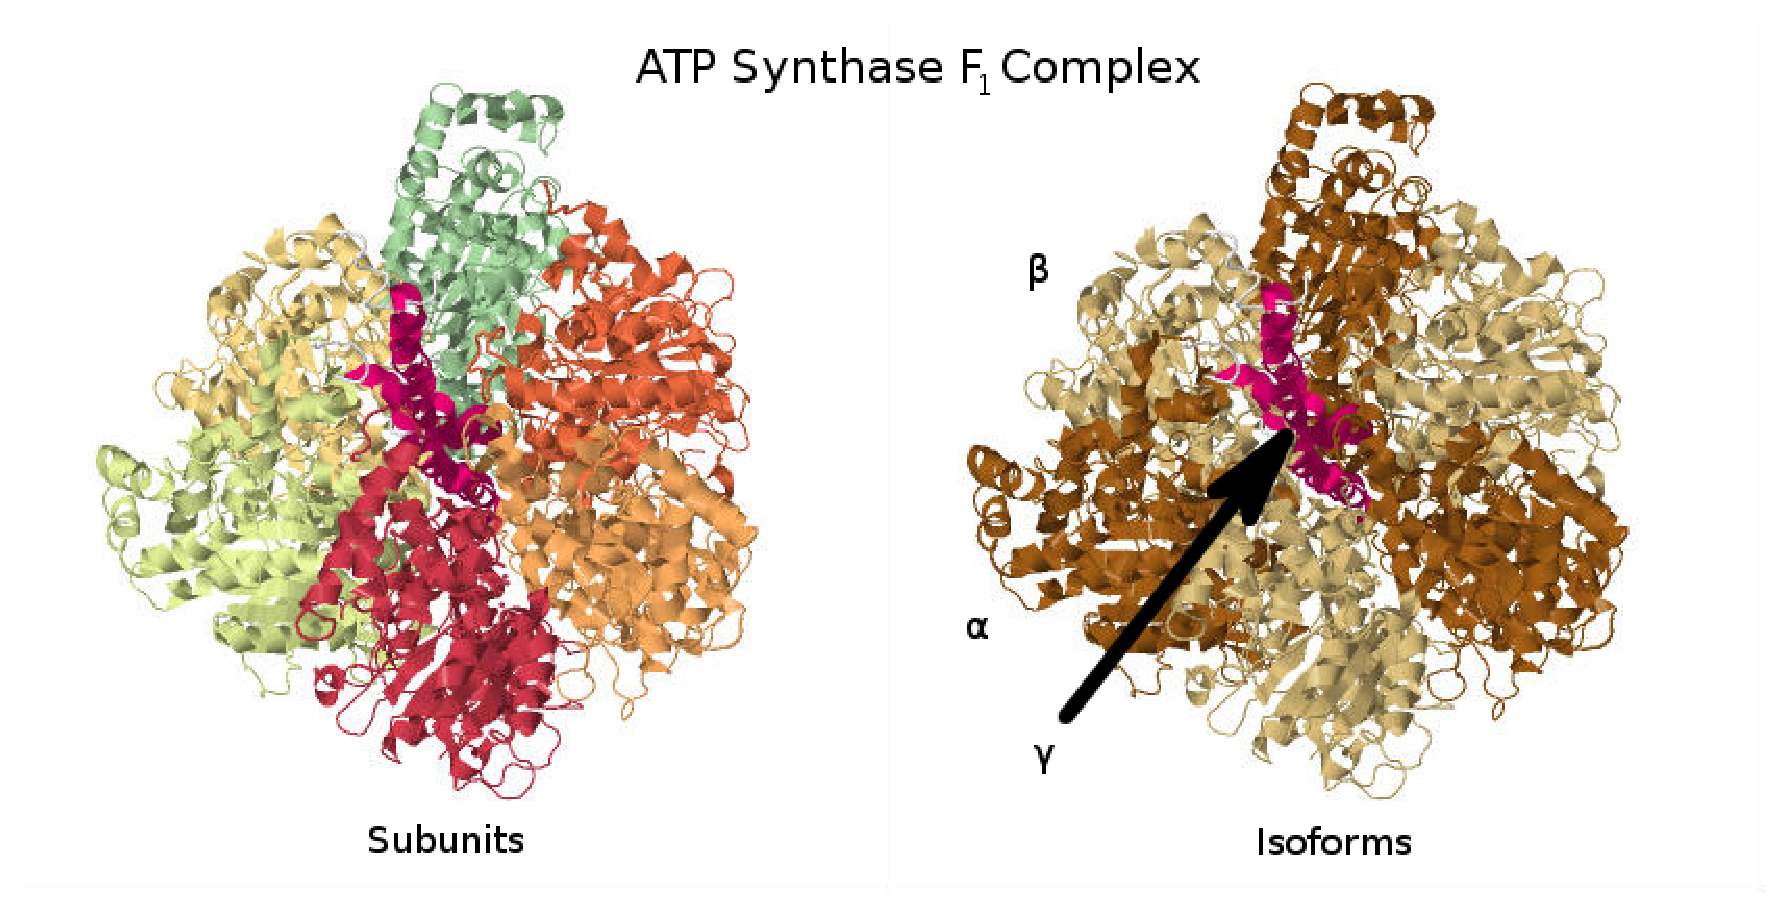
\includegraphics[clip=true,trim=0cm 0cm 0cm 0cm, width=12cm]{2F43}
\end{figure}

\emph{Assumption~\ref{ass:hierarchy}.}
The FALCON method used up until now performed a direct evaluation of
gene rule expression values---replacing gene names with their
expression values, ANDs with minimums, and ORs with sums, without
altering the logical expression of the GPR rule in any way---can lead
to some problems~\cite{Lee2012}. We illustrate this below, lower case
letters denote expression level (i.e. copy number of mRNA) of their
corresponding upper case letter, which denotes the gene name. The
$r_i$ are different reaction rules and the $e_i$ are the corresponding
estimated complex expression levels.

We need some way to guarantee that we don’t count anything twice or
more across disjunctions: \\
\begin{tabular}{cccccccc}
& $r_1$ & := & [A and B] or [A and C] & $\rightarrow$ & $e_1$  &=& min($a,b$) + min($a,c$) \\ 
& $r_2$ & := & [A and (B or C)]       & $\rightarrow$ & $e_2$  &=&  min($a, b + c$) 
\end{tabular} \\
Supposing A is the minimum, then if we just evaluate $r_1$ directly (a
rule in disjunctive normal form, or DNF), A will be counted twice.

Another possibility is divvying up expression for a rule in DNF. For
instance, in $r_1$ above, we could evaluate it as $e_1$ =
min($\frac{a}{2},b$) + min($\frac{a}{2},c$) to account for the
repeated use of $a$. However, other potential issues aside, we can see
that this can cause problems rather quickly. For instance, suppose $b
= a$ and $c = 0$; then min($a$,$b+c$) $=b=a$ appears to be correct,
not min($\frac{a}{2},b$) + min($\frac{a}{2},c$) = $\frac{a}{2} + 0$.

The modeling of enzyme complex copy number can be tackled by using
nested sets of subcomplexes; each enzyme complex consists of multiple
subcomplexes, unlesss it is only a single protein or family of protein
isozymes.  These subcomplexes are required for the enzyme complex to
function (AND relationships), and can be thought of as the division of
the complex in to distinct units that each have some necessary
function for the complex, with the exception that we do not keep track
of the multiplicity of subcomplexes within a complex since this
information is, in the current state of affairs, not always known.
However, there may be alternative versions of each functional set
(given by OR relationships). Eventually, this nested embedding
terminates with a single protein or set of peptide isoforms
(e.g. isozymes).  In the case of ATP Synthase, one of its functional
sets is represented by the $F_1$ subcomplex. The $F_1$ subcomplex
itself can be viewed as having two immediate subcomplexes: the single
$\gamma$ (axel) subunit and three identical subcomplexes each made of
an $\alpha$ and $\beta$ subunit. Each $\alpha\beta$ pair works
together to bind ADP and catalyze the reaction (cite). The
$\alpha\beta$ subcomplex itself then has two subcomplexes composed of
just an $\alpha$ subunit on the one hand and the $\beta$ subunit on
the other.  It is obvious that one of these base-level functional
subcomplexes (in this example, either $\gamma$ or $\alpha\beta$) will
be in most limited supply, and that it will best represent the overall
enzyme complex copy number (discounting the issues of multiplicity for
$\alpha\beta$, discussed above).

%
% Consider adding this as a Theorem/Proof:
%

The hierarhical structure just described, when written out in Boolean,
will give a rule in CNF (conjunctive normal form). This is because all
relations are ANDs (conjunctions), except possibly at the inner-most
subcomplexes that have alternative isoforms, which are expressed as
ORs (disjunctions). Since GPR rules alone only specify the
requirements for enzyme complex formation, we will see that not all
forms of boolean rules are equally useful in evaluating the enzyme
complex copy number, but we have established the assumptions in
Box~\ref{ECAssume} and an alternative and logically equivalent rule
\hl{(cite logic book)} under which we can estimate enzyme complex copy
number.

\label{ECAssume}
\begin{center}
\begin{tabular}{| p{14cm} |}
\hline
\textbf{Box ~\ref{ECAssume}. Assumptions in GPR-based Enzyme Complex Formation} \\
\hline
\begin{enumerate}
\item \begin{assume} \label{ass:expcorr}
Expression values are highly correlated with the copy numbers of their
corresponding peptide isoforms.
\end{assume}
\item \begin{assume} \label{ass:isozyme} 
Protein isoforms contributing to isozymes are considered part of the
same enzyme complex.
\end{assume}
\item \begin{assume} \label{ass:hierarchy}
Any enzyme complex can be described as a hierarchical subset of
(possibly redundant) subcomplexes; redundant subcomplexes, as
elaborated in (\ref{ass:nostoich}), are not currently modeled.
\end{assume}
\item \begin{assume} \label{ass:nostoich} 
Assume one copy of peptide per complex; exact isoform stoichiometry
is not considered.
\end{assume}
\item \begin{assume} \label{ass:sharing} 
With the exception of complexes having identical rules (i.e. the same
complex listed for different reactions), each copy of a peptide
is available for all complexes in the model.
\end{assume}
\item \begin{assume} \label{ass:active_site}
There is only one active site per enzyme complex.
\end{assume}
\item \begin{assume} \label{ass:holo} 
If a particular subcomplex can be catalyzed by A and it can also be
catalyzed by A and B (e.g. B acts as a regulatory unit, as in
holoenzymes), this just simplifies to A once expression values are
substituted in. Similarly, allosteric regulation is not
modeled. Relatedly, there are no NOT operations in GPR rules (just ANDs
and ORs).
\end{assume}
\item \begin{assume} \label{ass:chap} 
Enzyme complexes form without the assistance of protein chaperones and
formation is not coupled to other reactions.  
\end{assume}
\item \begin{assume} \label{ass:rate} 
Rate of formation and degradation of complexes doesn't play a role,
since we assume steady-state. 
\end{assume}
\end{enumerate} \\
\hline
\end{tabular}
\end{center}

There is no guarantee that a GPR rule has been written down with this
hierarchical structure in mind, though it is likely the case much of
the time as it is a natural way to model complexes.  However, any GPR
rule can be interpreted in the context of this hierarchical view due
to the existence of a logically equivlaent CNF rule for any non-CNF
rule, and it is obvious that logical equivalence is all that is
required to check for enzyme complex formation when exact isoform
stoichiometry is unknown.  As an example, we consider another common
formulation for GPRs, and a way to think about enzyme
structure---disjunctive normal form (DNF).  A DNF rule is a
disjunctive list of conjunctions of peptide isoforms, where each
conjunction is some variation of the enzyme complex due to
substituting in different isoforms for some of the required
subunits. A rule with a more complicated structure and compatible
isoforms across subcomplexes may be written more succinctinly in CNF,
whereas a rule with only very few alternatives derived from isoform
variants may be reprsented clearly with DNF.  In rare cases, it is
possible that a GPR rule is written in neither DNF or CNF, perhaps
because neither of these two alternatives above are stricly the case,
and some other rule is more succinct.

\emph{Assumptions~\ref{ass:nostoich},~\ref{ass:sharing}~and~\ref{ass:active_site}.}
One active site per enzyme complex implies a single
complex can only catalyze one reaction at a time. Multimeric complexes
with one active site per identical subunit would be considered as one
enzyme complex per subunit in this model.
Note that it is possible for an enzyme complex to catalyze different
reactions. In fact, some transporter complexes can transfer many
different metabolites \hl{across a lipid bilayer--up to}. Another
example is the ligation or hydrolysis of nucleotide, fatty acid, or
peptide chains, where chains of different length may all be substrates
or products of the same enzyme complex. While we do not explicitly
consider these in Algorithm~\ref{alg:ReductionToCNF}, these
redundancies are taken into account subsequently in
Algorithm~\ref{alg:FALCON}.  

What is currently not considered in our
process is that some peptide isoforms may find use in completely
different complexes, and in some cases, individual peptides may
have multiple active sites; in the first case, we assume an unrealistic case of
superposition where the isoform can simultaneously function in more
than one complex. The primary reason we have not tackled this problem
is because exact subunit stoichiometry of most enzyme complexes is not
accurately known, but an increasing abundance of data on BRENDA gives
some hope to this problem \hl{(cite BRENDA)}. Recent models such as the 
\emph{E. coli} M-E model \hl{(cite)} are beginning to incorporate 
enzyme complex stoichiometry into their GPRs, and we think this should
become standardized. For the second point, there are a
few enzymes where a single polpeptide may have multiple active sites
(e.g. fatty acid synthase), and this is not currently taken into 
account in our model. 

\emph{Assumption~\ref{ass:holo}.}
We do not make any special assumptions requiring symmetry of an isoform
within a complex. For instance, the example in
assumption~\ref{ass:holo} shows how you might have one
subcomponent composed of a single isoform, and another subcomponent
composed of that gene in addition to another isoform. In this case, it
is simply reduced to being the first gene only that is required, since
clearly the second is strictly optional. That isn't to say that the
second gene may not have some effect, such as (potentially) aiding in
structural ability or altering the catalytic rate, but it should have
no bearing on the formation of a functional catalytic
complex. Holoenzymes---enzymes with metabolic cofactors or protein
subunits that have a regulatory function for the complex---would
likely be the only situation where this type of rule might need to be
considered in more detail. But in the absence of detailed kinetic
information, this consideration not be useful, much like allosteric
regulation.

\emph{Assumptions~\ref{ass:chap}~and~\ref{ass:rate}.}
Due to the quickness, stability, and energetic favorability of enzyme
complex formation, the absence of chaperones or coupled metabolic
reactions required for complex formation may be reasonable
assumptions, but further research is warranted \cite{Karr2012}.
Additionally, as in metabolism, we assume a steady state for complex
formation, so that rate laws regarding complex formation aren't
needed. However, further research may be warranted to investigate the
use of a penalty for complex levels based on mass action and
protein-docking information. Requisite to this would be addressing
assumption~\ref{ass:nostoich}. It would be surprising if such a
penalty were significant, however, due to the cost this would imply
for many of the large and important enzyme complexes present in all
organisms.

\subsection{The Min Disjunction Algorithm Estimates \\Enzyme Complex Copy Number}

In the previous section, we showed that converting a rule to CNF is a
sound method to aid in the estimation of enzyme complex copy number.
However, attempting to symbolically convert the human ATP Synthase rule in
Human Recon 2 to CNF is computationally intractable due to an
exponential increase in memory \cite{Thiele2013}. Therefore, we use a
reduction rule that makes use of expression data, outlined below.
Note that the $AND$ and $OR$ notation is used to illustrate a
data structure that represents a set of literals that are
conjunctively or disjunctively joined together. The algorithm can be
represented as follows: \\

\pagebreak
\begin{Algorithm}
\label{alg:ReductionToCNF}
\begin{algorithmic}
\REQUIRE $g_i~s.t.~i \in{1, ..., m}$ are genes. 
\REQUIRE $x_i~s.t.~i \in{1, ..., n}$ are expressions in Boolean logic.
\WHILE{$rule \neq AND(o_1,...,o_p)$ where each $o_i$ has the form: $OR(...,g_j,...)~s.t.~j \leq m$}
  \STATE $\mathbf{1}$: check for sequence of ANDs of literals (genes)\\ 
    \hspace{4.8 mm} $\rightarrow$ reduce to gene with minimum expression 
  \STATE $\mathbf{2}$: Distribute ORs over ANDs, e.g.: $(x_1 \land x_2) \lor (x_3 \land x_4)$ \\ 
    \hspace{4.8 mm} $\rightarrow (x_1 \lor x_3) \land (x_1 \lor x_4) \land (x_2 \lor x_3) \land (x_2 \lor x_4)$
  \STATE $\mathbf{3}$: Change adjacent gene arguments to sets, e.g: \\
    \hspace{4.8 mm} $g_1 \land g_2 \rightarrow AND(g_1,g_2)$;  \\
    \hspace{4.8 mm} $g_1 \land AND(g_2,g_3) \rightarrow AND(g_1,g_2,g_3)$ 
\ENDWHILE
\ENSURE $o_{min}$ where $o_{min}$ has the form: $OR(g_1,...,g_m)$
\end{algorithmic} 
\end{Algorithm}

The third step greatly simplifies numeric manipulations and checking
for the terminating condition. Please see below for the code for the
core part of the algorithm. Now we show that the reduction step does
not change the desired result of the algorithm.

\begin{Theorem}
\label{thm:ReductionToCNF}
Algorithm~\ref{alg:ReductionToCNF} returns the disjunction with
minimum expression value among all disjunctions of a rule in CNF.
\end{Theorem}

\begin{proof}
The third step in the while-loop does not affect the
underlying logic, so we only need to consider the effect of step one
on step two.  Let us first consider when expressions $x_1, ..., x_4$
are all literals in step two to cover the most complex case, and that
$x_i^{(e)}$ denotes the expression measurement for gene $x_i$. Assume
WLOG that $x_1 \lor x_3$ attains the minimum expression among the
disjunctions. Then we have:

\begin{align*}
&x_{1}^{(e)} + x_{3}^{(e)} \leq x_{1}^{(e)} + x_{4}^{(e)} \Rightarrow x_{3}^{(e)} \leq x_{4}^{(e)} \\
&x_{1}^{(e)} + x_{3}^{(e)} \leq x_{2}^{(e)} + x_{3}^{(e)} \Rightarrow x_{1}^{(e)} \leq x_{2}^{(e)} 
\end{align*}

Applying this result in conjunction to step one in the while-loop to
the original expression, $(x_1 \land x_2) \lor (x_3 \land x_4)$, we
immediately arrive at $(x_1) \lor (x_3)$, which gives our originally
assumed minimum. To show that this result doesn't depend on the $x_i$
being literals, merely consider repeating this process recursively for
each $x_i$ that is not a literal to arrive at two different
evaluations for $x_i^{(e)}$ (one where each evaluation is done with reduction, 
and one where we evaluate entirely without reduction). 
Since the process cannot continue
indefinitely, eventually there is a base case involving only literals,
and the above result shows that, at each step, as we propagate back,
both evaluations will be identical. The desired result is obtained
because Algorithm~\ref{alg:ReductionToCNF} without step one simply yields CNF,
and it follows that adding step one will yield the disjunction with 
minimum expression value of the rule in CNF.
\end{proof}

The method presented here for enzyme complex copy number estimation
can be used as a stand-alone method, as long as GPR rules from a
metabolic reconstruction are present. For instance, it may not always
be desirable to directly compute a flux. As an example, the relative
copy number of enzyme complexes present in secretions from various
biological tissues, such as milk or pancreatic secretions, may still
be of interest even without any intracellular flux data.  Perhaps more
importantly, this approach to estimating relative complex levels can
be employed with regulatory models such as PROM or other regulatory
network models that can estimate individual gene expression levels at
time $t+1$ given the state of the model at a time $t$ (\hl{cite PROM,
some other bayesian regulatory/signalling model}).

\subsection{Formulation with Automatic Normalization and Fast Direction Assignment}
Unlike the original formulation of FALCON, we employ a normalization variable $n$ in the problem
to find the most agreeable scaling of expression data. Additional technical constraints not shown
from Linear Fractional Programming (LFP) require $n$ to be non-zero \cite{Boyd2004}. The
LFP shown below can be converted to a linear program by the Charnes-Cooper transformation.
However, in the first iteration of the algorithm, we ask the user to
specify an enzyme-associated reaction $v_{scale}$ and associated flux
constant $c_{scale}$ so that when the $e_i$ are scaled, we have
$e_{scale} = v_{scale} = c_{scale}$. This guarantees that the
optimization problem will yield a non-zero flux vector and also helps
to put the fluxes and expression measures on the same order of
magnitude, which can be important for numerical stability.

Additionally, the original formulation
used repeated iterations of FVA (Flux Variability Analysis). This is a very costly procedure. 
To address this, we convert the model to an irreversible model, where each reversible flux $v_j$
in the original model is split into a forward and backward reaction that take strictly positive
values: $v_{j,f}$ and $v_{j,b}$. To keep track of how many reactions
are currently irreversible, we use the variables $rxns_{irrev}$ and
$rxns_{irrev,prior}$. The algorithm terminates when no more reactions
can be found to have a definite direction.  Given indexed families
$R_i$ of reactions with the identical gene rules in each set and
estimated expression values $e_i$, we can describe the new problem as:

\pagebreak
\begin{Algorithm}[FALCON]
\label{alg:FALCON}
\begin{algorithmic}
\WHILE{$rxns_{irrev} > rxns_{irrev,prior}$}
  \STATE {$rxns_{irrev,prior} := rxns_{irrev}$}
  \IF {first iteration}
  \STATE {Constrain a user-specified flux $v_{scale} = c_{scale}$} 
  \INDSTATE {(either forward or backward) to a nonzero value.}
  \STATE {Scale $e_i$ so that $e_{scale} = v_{scale} = c_{scale}$.}
  \ELSE 
  \STATE {Restore original constraints for user specified flux.}
  \ENDIF
  %\begin{align*}
  \STATE {Call LP Solver:}
  \INDSTATE $\textnormal{minimize}\ \sum^N_{i=1}\frac{d_i}{n \sigma_i}$  \\
  \INDSTATE s.t. \\
  \INDSTATE $\forall i: -d_i \leq \sum_{j \in R_i}(v_{j,f} + v_{j,b}) - n e_i \leq d_i$ \\
  \INDSTATE $d_i, v_{j,f}, v_{j,b} \geq 0$ \\
  \INDSTATE $n > 0$
  %\end{align*}
  \FORALL {$v_{i,f} > 0$}
  \IF {$v_{i,f} = v_{i,b}$}
  \STATE {Constrain $v_{i,f}, v_{i,b} = 0$.}  
  \STATE {$rxns_{irrev}$++}
  \ENDIF
  \IF {$v_{i,b} > 0$}
  \STATE {Constrain the smaller of $v_{i,f}$ and $v_{i,b}$ to be $0$.}  
  \STATE {$rxns_{irrev}$++}
  \ENDIF
  \ENDFOR
\ENDWHILE
\end{algorithmic}
\end{Algorithm}
Note that as in the original FALCON paper, $\sigma_i$ is an optional weighting of variation
in biological or technical replicates. 

In the original formulation, FVA uses an objective with a $-1$ or $+1$ for each reversible reaction 
with all other reactions having a 0. If having a non-zero flux in the negative or positive direction
does not increase the residuals' magnitude (which is the objective of the FALCON problem), then 
the reaction is made irreversible for subsequent iterations. Eventually this process terminates
when the number of reversible reactions remains constant. 

During each iteration we allow flux through both $v_f$ and $v_b$; if one of these is is greater 
than the other, then the lesser flux is constrained to be zero in subsequent iterations. What
can be done in practice is to pick a parameter $\alpha \in [0.5,1)$ so that if
$\frac{v_f}{v_f+v_b} > \alpha$ then $v_b$ is constrained to be 0 subsequently. This parameter could
also be changed as iterations progress, but so far there appears to be no advantage to using
anything other than $0.5$ (larger values terminate more quickly, but with slightly fewer reaction
directions determined).

If $v_f = v_b$ after an iteration, we constrain both reactions to be zero, since this
is a futile cycle. Otherwise, the flux through these reactions may be inadvertently affecting
the obective. If we don't do this, we actually see about 100 fewer reactions active in an FALCON run.
The disadvantage is that the time for completing FALCON goes up from about 70s to 200s on a recent
AMD Athlon Magny-Cours system running the Gurobi 5.1 solver. This is still a major improvement 
in efficiency over the FVA method, which could take several hours per Human Recon 2 FALCON run.

Further work on improving convergence speed should be kept in mind, or
at least, making use of prior FALCON flux estimations (see the section
below about mutational models and epistasis) to give the algorithm a
warm start.  Regularization is one technique that may prove useful in
attaining better convergence speed by somewhat simplifying the flux
vector; regularization has been found to be a biologically important
objective in microbes (cite Uwe Sauer).


%Make performance tables like this? 
\begin{table}[!t]
\processtable{This is table caption\label{Tab:01}}
{\begin{tabular}{llll}\toprule
head1 & head2 & head3 & head4\\\midrule
row1 & row1 & row1 & row1\\
row2 & row2 & row2 & row2\\
row3 & row3 & row3 & row3\\
row4 & row4 & row4 & row4\\\botrule
\end{tabular}}{This is a footnote}
\end{table}

\end{methods}

\begin{figure}[!tpb]%figure1
%\centerline{\includegraphics{fig01.eps}}
\caption{Caption, caption.}\label{fig:01}
\end{figure}

\begin{figure}[!tpb]%figure2
%\centerline{\includegraphics{fig02.eps}}
\caption{Caption, caption.}\label{fig:02}
\end{figure}

\section{Discussion}

Text Text Text Text Text Text  Text Text Text Text Text Text Text Text Text  Text Text Text Text Text Text. Figure \ref{fig:02} shows that the above method  Text Text Text Text  Text Text Text Text Text Text  Text Text.  \citealp{Boffelli03} might want to know about  text text text text
Text Text Text Text Text Text  Text Text Text Text Text Text Text Text Text  Text Text Text Text Text Text. Figure \ref{fig:02} shows that the above method  Text Text Text Text  Text Text Text Text Text Text  Text Text.  \citealp{Boffelli03} might want to know about  text text text text
Text Text Text Text Text Text  Text Text Text Text.




Table~\ref{Tab:01} shows that Text Text Text Text Text  Text Text Text Text Text Text. Figure \ref{fig:02} shows that
the above method Text Text. Text Text Text  Text Text Text Text Text Text. Figure \ref{fig:02} shows that
the above method Text Text. Text Text Text  Text Text Text Text Text Text. Figure \ref{fig:02} shows that
the above method Text Text.









%%%%%%%%%%%%%%%%%%%%%%%%%%%%%%%%%%%%%%%%%%%%%%%%%%%%%%%%%%%%%%%%%%%%%%%%%%%%%%%%%%%%%
%
%     please remove the " % " symbol from \centerline{\includegraphics{fig01.eps}}
%     as it may ignore the figures.
%
%%%%%%%%%%%%%%%%%%%%%%%%%%%%%%%%%%%%%%%%%%%%%%%%%%%%%%%%%%%%%%%%%%%%%%%%%%%%%%%%%%%%%%






\section{Conclusion}

(Table~\ref{Tab:01}) Text Text Text Text Text Text  Text Text Text Text Text Text Text Text Text  Text Text Text Text Text Text. Figure \ref{fig:02} shows that the above method  Text Text Text Text  Text Text Text Text Text Text  Text Text.  \citealp{Boffelli03} might want to know about  text text text text
Text Text Text Text Text Text  Text Text Text Text Text Text Text Text Text  Text Text Text Text Text Text. Figure \ref{fig:02} shows that the above method  Text Text Text Text  Text Text Text Text Text Text  Text Text.  \citealp{Boffelli03} might want to know about  text text text text
Text Text Text Text Text Text  Text Text Text Text Text Text Text Text Text  Text Text Text Text Text Text. Figure \ref{fig:02} shows that the above method  Text Text Text Text  Text Text Text Text Text Text  Text Text.



Text Text Text Text Text Text  Text Text Text Text Text Text Text Text Text  Text Text Text Text Text Text. Figure \ref{fig:02} shows that the above method  Text Text Text Text  Text Text Text Text Text Text  Text Text.  \citealp{Boffelli03} might want to know about  text text text text





\begin{enumerate}
\item this is item, use enumerate
\item this is item, use enumerate
\item this is item, use enumerate
\end{enumerate}

Text Text Text Text Text Text  Text Text Text Text Text Text Text Text Text  Text Text Text Text Text Text. Figure \ref{fig:02} shows that the above method  Text Text Text Text  Text Text Text Text Text Text  Text Text.  \citealp{Boffelli03} might want to know about  text text text text
Text Text Text Text Text Text  Text Text Text Text Text Text Text Text Text  Text Text Text Text Text Text. Figure \ref{fig:02} shows that the above method  Text Text Text Text  Text Text Text Text Text Text  Text Text.  \citealp{Boffelli03} might want to know about  text text text text
Text Text Text Text Text Text  Text Text Text Text Text Text Text Text Text  Text Text Text Text Text Text.






Text Text Text Text Text Text  Text Text Text Text Text Text Text Text Text  Text Text Text Text Text Text. Figure \ref{fig:02} shows that the above method  Text Text Text Text

